\section{Development} % Major section

As I said in Section \ref{sec:tec} in this work we have HTML, CSS and JS.

The function of HTML is place the elements that the JS will change, and the CSS will stylize. This is the case of the Youtube box and buttons. The function of CSS is to stylize the page, and apply some cool effects, like round corners and place the wallpaper. The function of JS is to change elements of JS. When I press a button to move to the next slide, the JS will change the background and play another music of Youtube.

It is a very simple program.

%------------------------------------------------

\subsection{Images} % Sub-section

\begin{figure}[h]
\centering
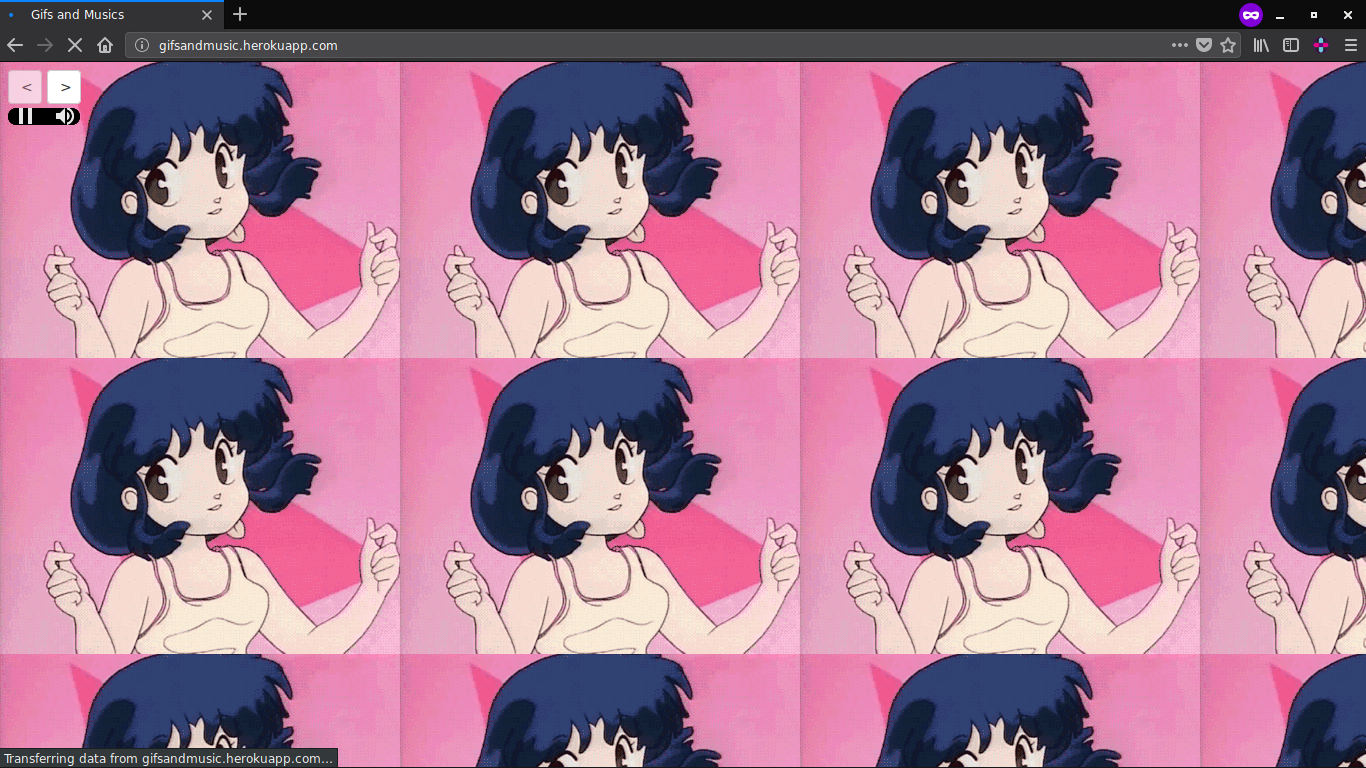
\includegraphics[scale=.37]{1.png}
\caption{This is the first gif you will see in the website.}
\label{figure1}
\end{figure}

Besides the wallpaper, in Figure \ref{figure1} you can see in the north-west region two buttons and one black box.

The function of those buttons is to change to the next pair of gif and music. The reason why de left button is disabled is because this is the first pair, in other words, there is no pair behind the first one.

The function of the black box is to play a Youtube song, where you can pause and mute the music.

\begin{figure}[h]
\centering
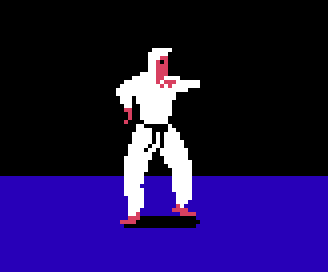
\includegraphics[scale=.37]{2.png}
\caption{Another pair of gif and music.}
\label{figure2}
\end{figure}

In Figure \ref{figure2} you can see that the first button isn't disabled anymore, that can be explained because there is a pair behind this current pair.

\begin{figure}[H]
\centering

\includegraphics[scale=.37]{3.png}
\caption{Example of last pair of gif and music.}
\label{figure3}
\end{figure}

The reason why the right button is disabled in Figure \ref{figure3} is obvious, it is because this is the current last pair of gif and music.

\subsection{Run}

You have two options to run this program.

\subsubsection{Online}
The first one is the simplest and basically you just need to access the published website \cite{heroku}.

\subsubsection{Local}
Or you can follow these steps of cloning my Github repo \cite{craviee}
\begin{enumerate}

	\item Open a Linux terminal
	
	\item Type: git clone https://github.com/craviee/GifsAndMusic.git
	
	\item Go to the folder you just downloaded and go to html folder
	
	\item Open the home.html with your favourite browser
	
\end{enumerate}

%----------------------------------------------------------------------------------------
%	MAJOR SECTION X - TEMPLATE - UNCOMMENT AND FILL IN
%----------------------------------------------------------------------------------------

%\section{Content Section}

%\subsection{Subsection 1} % Sub-section

% Content

%------------------------------------------------

%\subsection{Subsection 2} % Sub-section

% Content